\documentclass[review,supplement,hidelinks,onefignum,onetabnum]{siamart251216}
% SIAM format only; mathematical source remains English V12 Final.
\usepackage{microtype,xurl}
\usepackage{amsfonts,amssymb,mathtools,bm}
\usepackage{graphicx,booktabs,enumitem,float,tabularx,placeins}
\graphicspath{{../../paper/}{../../supplementary/}}
\usepackage[numbers,sort&compress]{natbib}
\newsiamremark{assumption}{Assumption}
\newsiamremark{remark}{Remark}
\headers{When Can Markets Crash Without News?}{Siyuan Ye}
\title{When Can Markets Crash Without News?}
\author{Siyuan Ye\thanks{Independent Researcher.}}
\hypersetup{pdftitle={When Can Markets Crash Without News?},pdfauthor={Siyuan Ye}}
\setlength{\emergencystretch}{1em}
% The unmodified online class's two-line running head exceeds its 10pt preset.
\setlength{\headheight}{14pt}
\newcommand{\R}{\mathbb{R}}
\newcommand{\Cris}{\mathcal{C}}
\newcommand{\calK}{\mathcal{K}}
\newcommand{\calA}{\mathcal{A}}
\newcommand{\dd}{\,\mathrm{d}}
\newcommand{\one}{\mathbf{1}}
\newcommand{\pos}[1]{[#1]_+}
\newcommand{\Law}{\mathcal{L}}
\newcommand{\totv}{\operatorname{TV}}

\begin{document}
\maketitle
\section{Scope of the supplement}
These panels and the earlier nonoptimal two-day witness are preserved for replication and illustration. They are not independent estimates of real market risk. All mathematical claims and the improved interval-certified construction appear in the main manuscript.
\section{Earlier exploratory two-day execution}

The preceding theorems form a hierarchy of \emph{necessary} tests. Passing the rolling-band bound, the scalar selling-rate test, the dollar-closure preconditioning test, and the cut-capacity test still does not prove a path exists. We therefore turn from exclusion and lower bounds to a constructive example that enforces the constraints \emph{simultaneously}. To test repeated \emph{partial-coverage} lower-limit closes, we constructed a continuous $N=10$, $k=9$ example in the $g(S)\equiv\eta$ market. The nine targets use symmetric $\pm3\%$ proportional bands; the compensator uses a wider symmetric $\pm25\%$ band. These are \emph{hypothetical normalized assets}, not calibrated TSE stocks. Set $F=\eta=1$, $\rho=0.4$, equal session lengths $\tau_1=\tau_2=20$, and a common gross share-rate limit $\bar v=1$.

Write $S_1=\cdots=S_9=x(t)$ and $S_{10}=y(t)$. On each session let $x(t)$ be a continuous piecewise-linear path: it rises to a first-session plateau $h_1$ then closes at $0.97$, rises to a second-session plateau $h_2=0.995$ then closes at $0.97^2=0.9409$. All ramps last $0.7$ trading-time units. Dollar pairing uniquely determines the compensator's ODE via
\begin{equation}\label{eq:multiday-witness-ode}
 u(t)=x(t)[\dot x(t)+\rho(x(t)-1)],\qquad
 \dot y=-\rho(y-1)-\frac{9u(t)}{y(t)},\quad y(0)=1.
\end{equation}
The first plateau $h_1\approx1.0142982125$ is selected from the \emph{exact piecewise-polynomial} equation
\begin{equation}\label{eq:multiday-closed}
 X_i(T_2)=\frac{x(T_2)^2-1}{2}+\rho\int_0^{T_2}x(t)[x(t)-1]\dd t=0,
 \quad i=1,\ldots,9.
\end{equation}
Because $\dot X_{10}=-9\dot X_1$, the compensator's terminal executed-dollar balance closes as well. Independent high-accuracy ODE and Runge--Kutta integrations agree for $y(T_2)$ to approximately $2\times10^{-12}$; band and rate slack were checked on a dense time grid. These numerical checks are an explicit \emph{witness}, not a proof of general $N$-asset sufficiency or a certified interval-enclosure theorem.

\begin{table}[tbp]\centering\small
\caption{Two-session $N=10$ deterministic closing-limit witness (normalized units). Day 1 and Day 2 target losses are $3\%$ each relative to the reset reference; the terminal systemic functional is smaller because the compensator rises.}\label{tab:multiday-witness}
\begin{tabular}{@{}p{.48\linewidth}r@{}}\toprule
Quantity & Verified value \\\midrule
Nine target closing prices, session 1 / session 2 & $0.970000$ / $0.940900$\\
Compensator closing prices, session 1 / session 2 & $1.228104$ / $1.417574$\\
Maximum individual gross executed-share rate & $0.680780 < \bar v=1$\\
Target executed-dollar balance, day 1 / day 2 & $+0.078235$ / $-0.078235$\\
Maximum absolute terminal net-dollar balance & $< 7\times10^{-15}$\\
Total paired-dollar turnover / largest gross share sales & $2.59310$ / $1.46241$\\
Terminal $\Cris_{0.9}(T_2)$ / breadth loss $Q_{0.9}(T_2)$ & $0.019932$ / $0.060918$\\
\bottomrule\end{tabular}
\end{table}

\begin{figure}[tbp]\centering
 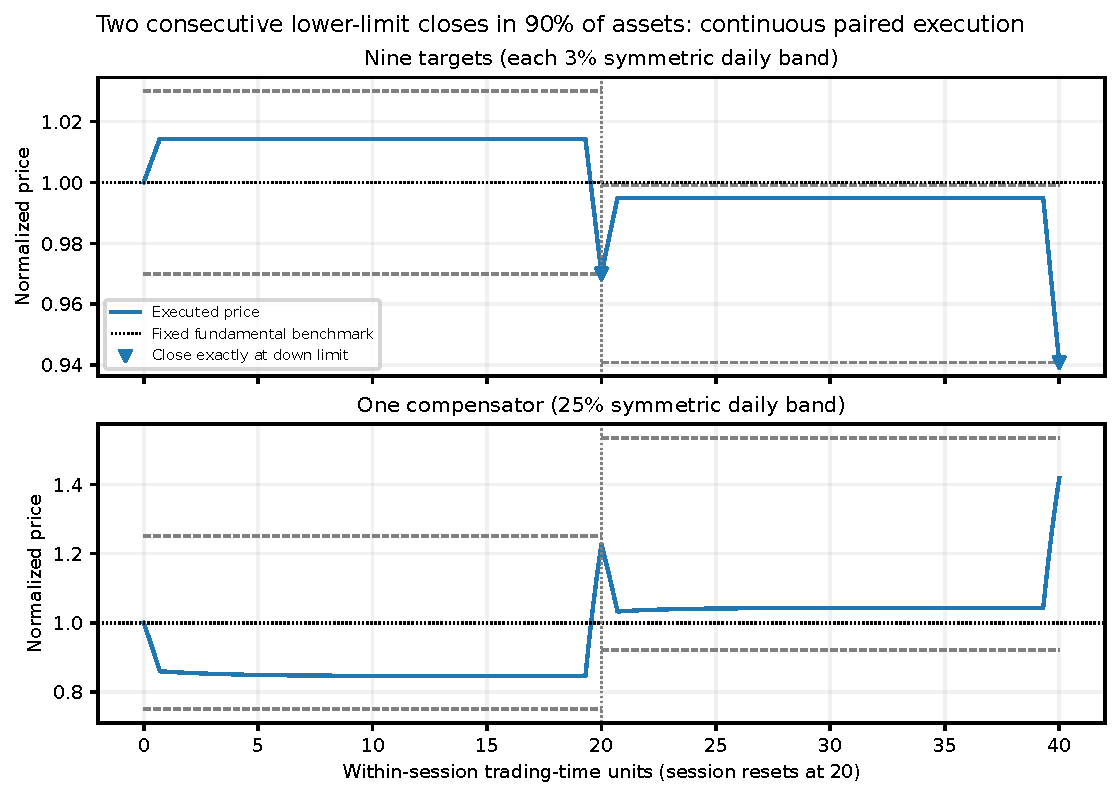
\includegraphics[width=.94\linewidth]{figures/multiday_streak_witness.pdf}
 \caption{\textbf{Repeated partial-coverage lower-limit closing prices under rolling daily bands.} The same nine target assets close at their 3\% lower limits twice. The tenth, higher-band compensating asset stays within its own 25\% limits. The displayed paths contain no instantaneous trades. The horizon and bands are specified model inputs, not observations.}\label{fig:streak-witness}
\end{figure}
\begin{figure}[tbp]\centering
 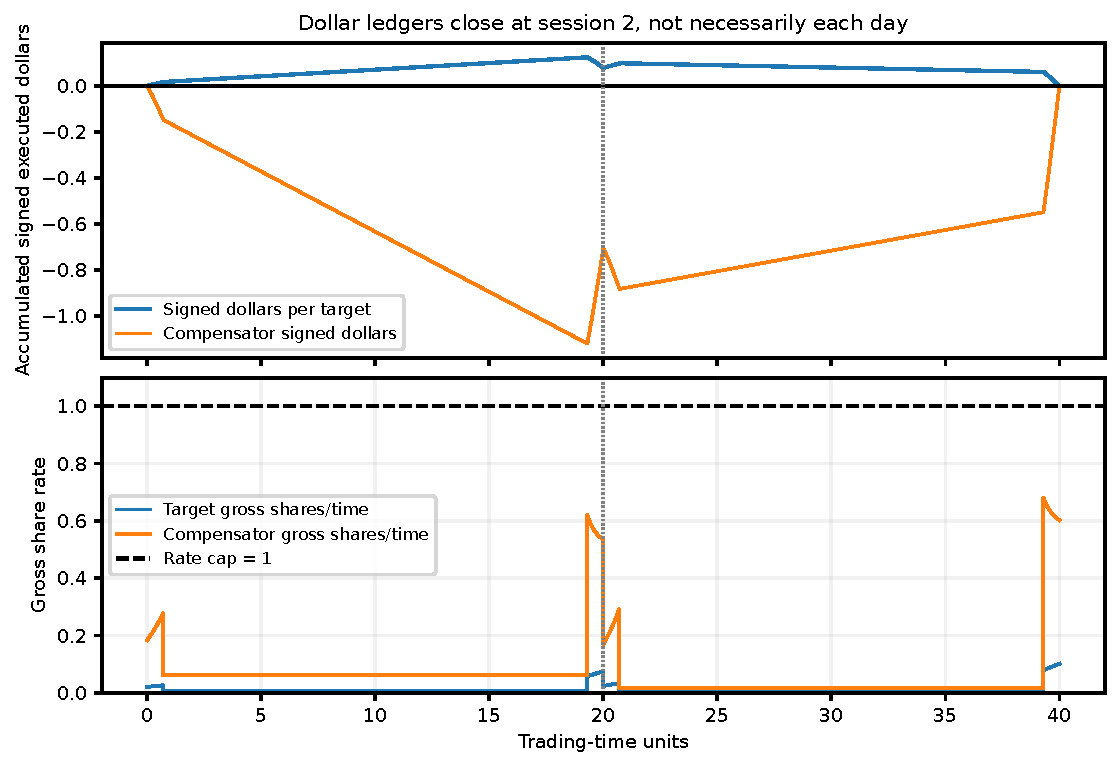
\includegraphics[width=.94\linewidth]{figures/multiday_ledgers_and_rates.pdf}
 \caption{\textbf{Trading ledgers and gross-rate check for the same two-session witness.} The first session builds positive net dollar flow in the targets; the second reverses it, leaving every asset's final signed-dollar balance zero. Gross rates remain below the imposed share-rate limit; dollar balance is enforced continuously, not just at maturity.}\label{fig:streak-ledger}
\end{figure}

The example proves neither a trader's incentive to undertake the sequence nor a \emph{locked} limit-down order book. It does show numerically that rolling bands, finite executed-share rates, no fundamental-news shocks, and terminal dollar closure can be compatible with \emph{multiple} lower-limit closes in a broad subset of assets. For a crisis threshold, the breadth requirement alone does not suffice: for this path $Q_{0.9}(T_2)=0.060918$ but the average-loss restriction binds, giving $\Cris_{0.9}(T_2)=0.019932$ (thus, for example, $\delta=0.015$ is reached). No claim of an exact minimum rate, minimum turnover, or equilibrium occurrence follows.



\section{Other diagnostic displays}
\begin{figure}[tbp]
\centering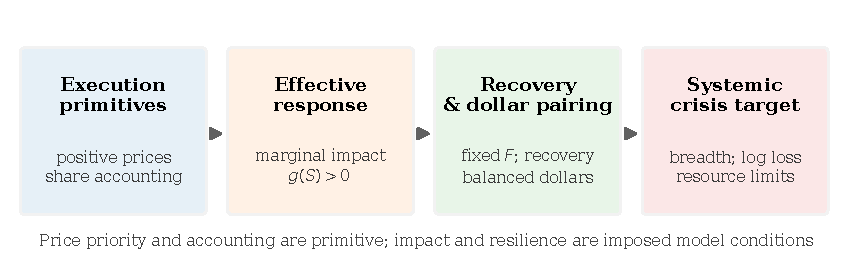
\includegraphics[width=.99\linewidth]{figures/market_specification.pdf}
\caption{\textbf{One explicitly defined ideal market.} Price priority, signed-share accounting, effective price impact, resilience, and paired-dollar trading have distinct mathematical roles. All quantitative panels in this paper are illustrations of this specified model rather than observations of a live order book.}\label{fig:market}
\end{figure}
\begin{figure}[tbp]
\centering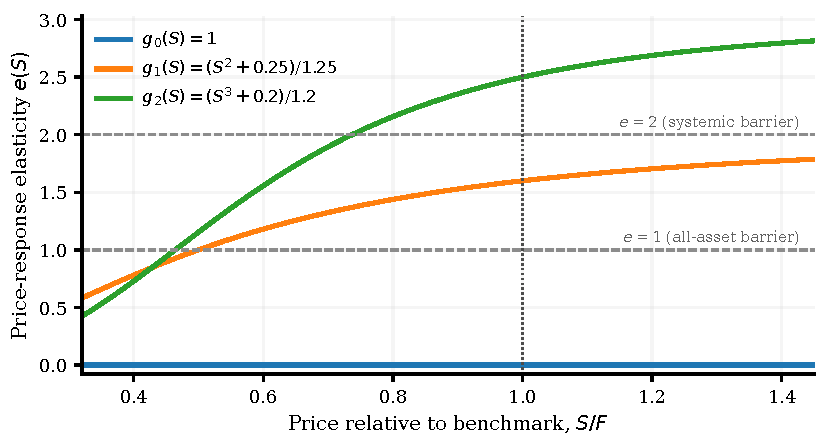
\includegraphics[width=.79\linewidth]{figures/elasticity_examples.pdf}
\caption{\textbf{Local elasticity of three positive, smooth, non-power-law impact functions.} The dotted vertical line marks the common initial price $S=F$. The global elasticity-barrier theorems in the main manuscript require their elasticity inequalities throughout the \emph{relevant attainable price region}; a value at $F$ alone gives no global classification. This is a formula-based illustration, not empirical market depth.}\label{fig:elasticity}
\end{figure}
\begin{figure}[t]
\centering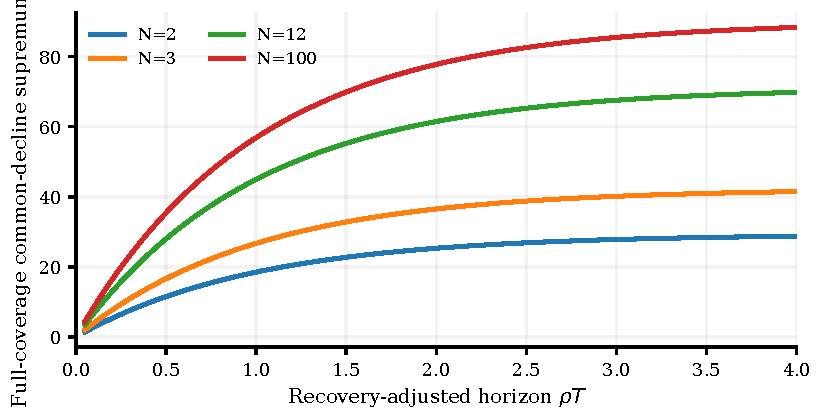
\includegraphics[width=.78\linewidth]{figures/full_coverage_threshold.pdf}
\caption{\textbf{A sharp, model-specific common-decline boundary.} For $g=\eta$ and $k=N$, the upper envelope of the common simple-price decline is $100(1-e^{-\delta_{\rm crit}})\%$. Every strictly smaller log-loss threshold is reachable with some finite budget; the boundary itself is not attained with strictly positive prices. This is not a probability curve.}\label{fig:sharp}
\end{figure}
\begin{figure}[tbp]
\centering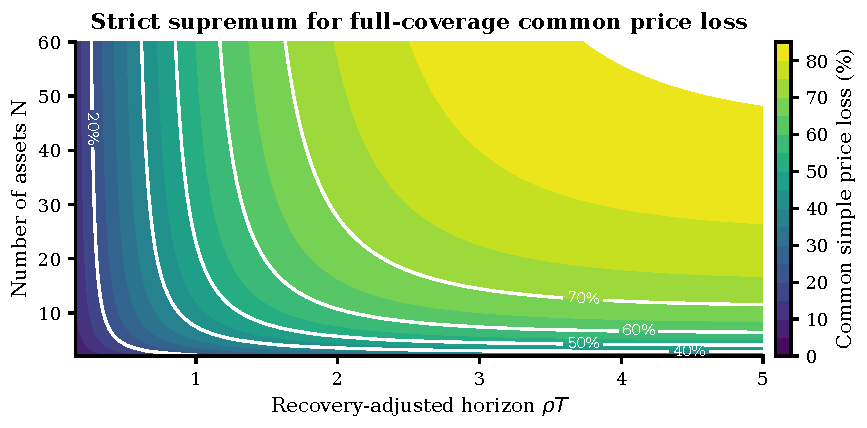
\includegraphics[width=.83\linewidth]{figures/all_asset_boundary_heatmap.pdf}
\caption{\textbf{The full-coverage boundary across asset count and recovery time.} Color reports $100(1-e^{-\delta_{\rm crit}(N,T)})$, the supremum of simultaneous \emph{simple-price} losses for constant per-share impact with individually closed terminal dollar flows. No probability, observed drawdown, or finite-budget optimum is inferred.}\label{fig:heatmap}
\end{figure}
\begin{figure}[tbp]
\centering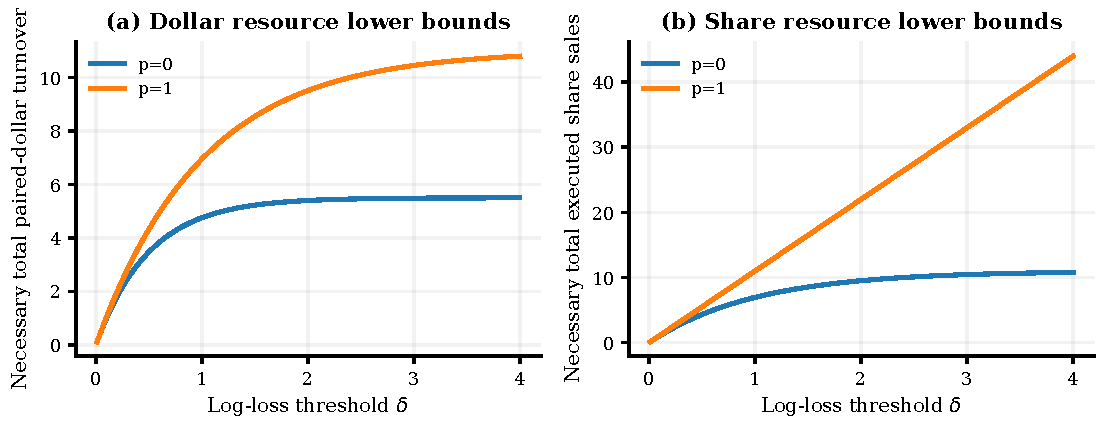
\includegraphics[width=.96\linewidth]{figures/resource_lower_bounds.pdf}
\caption{\textbf{General necessary resource floors illustrated for the power-response family.} With $F=\eta=1$ and $k=11$, the curves evaluate $k\int_{e^{-\delta}}^1 S/g(S)\dd S$ (dollars) and $k\int_{e^{-\delta}}^1 1/g(S)\dd S$ (shares), for $p=0,1$. The bounds are \emph{not} the optimal execution cost and do not establish reachability.}\label{fig:resource}
\end{figure}
\begin{figure}[tbp]
\centering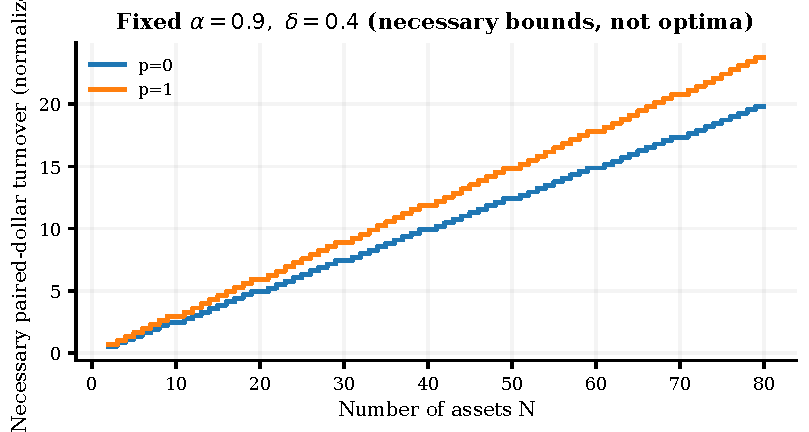
\includegraphics[width=.78\linewidth]{figures/resource_scaling_N.pdf}
\caption{\textbf{Dependence on asset number of the necessary dollar-resource bound.} The experiment copies per-asset benchmark price and response parameters, fixes $\alpha=0.9$ and $\delta=0.4$, and increases the number of assets $N$. The steps arise from the discrete coverage count $\lceil\alpha N\rceil$. It is not a capitalization-scaled prediction for an actual stock index.}\label{fig:nscale}
\end{figure}
\begin{figure}[tbp]\centering
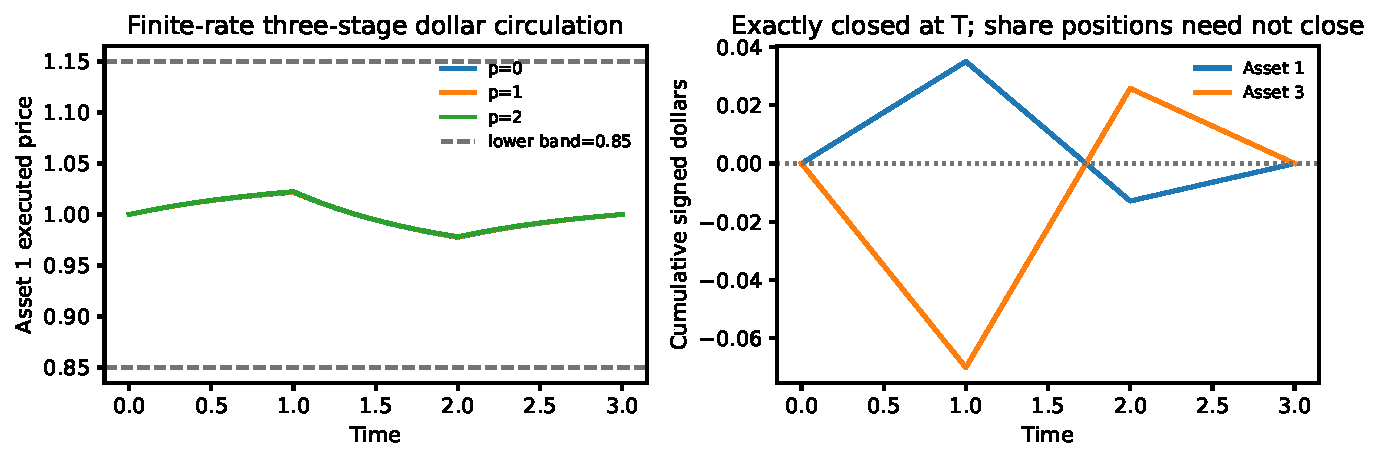
\includegraphics[width=.97\linewidth]{figures/bounded_rate_continuous_path.pdf}
\caption{\textbf{A new bounded-rate, terminally dollar-closed path (not a pulse approximation).} For $N=3$, $T=3$, $a=.035$, $F=\rho=\eta=1$, and $u=(1,1,-2)$, the price trajectories under $p=0,1,2$ share the same absolutely continuous dollar-rate signal; right panel shows dollar ledgers that close exactly. The peak per-asset gross share rate is below $0.15$, and all prices remain inside a $\pm15\%$ band.}\label{fig:continuous}
\end{figure}
\begin{figure}[tbp]\centering
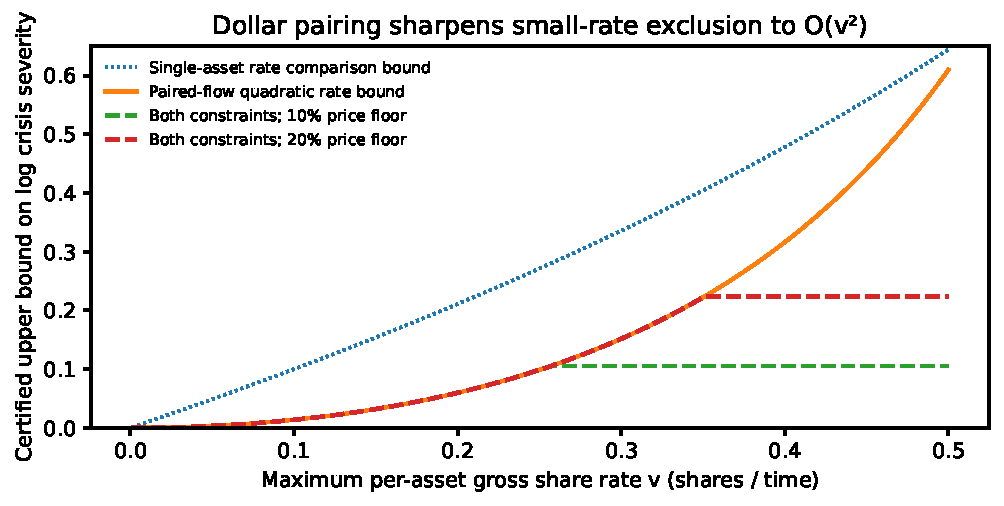
\includegraphics[width=.78\linewidth]{figures/rate_and_price_limit_bounds.pdf}
\caption{\textbf{Exclusion certificates, not exact reachable maxima.} For $g=\eta=F=\rho=1$ and $T=3$, a paired-flow quadratic estimate improves the single-price comparison at small rates; a single-session lower price band provides an additional hard ceiling. Neither curve reports optimal crisis control or an observed market frequency.}\label{fig:regulation}
\end{figure}
\begin{figure}[tbp]\centering
 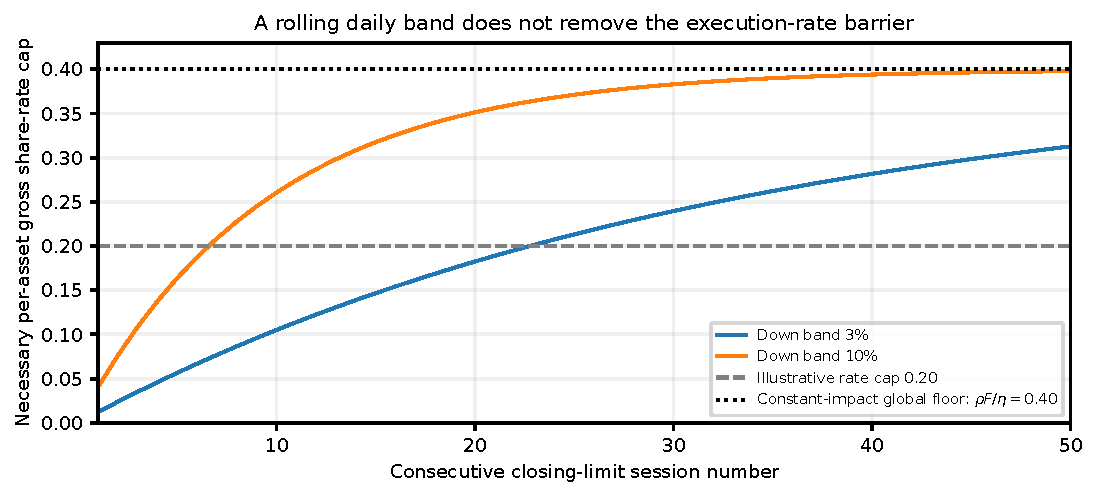
\includegraphics[width=.88\linewidth]{figures/multiday_rate_frontier.pdf}
 \caption{\textbf{Necessary gross share-rate floor for repeated lower-limit closes.} The scalar constant-impact necessary-rate formula in the main manuscript in the scalar constant-impact comparator, $F=\eta=1$, $\rho=0.4$, $\tau=20$. These are \emph{necessary} per-asset rates; paired execution, available inventory, and the compensator's own daily band can make the actual market threshold higher.}\label{fig:streak-rate}
\end{figure}
\begin{figure}[tbp]\centering
 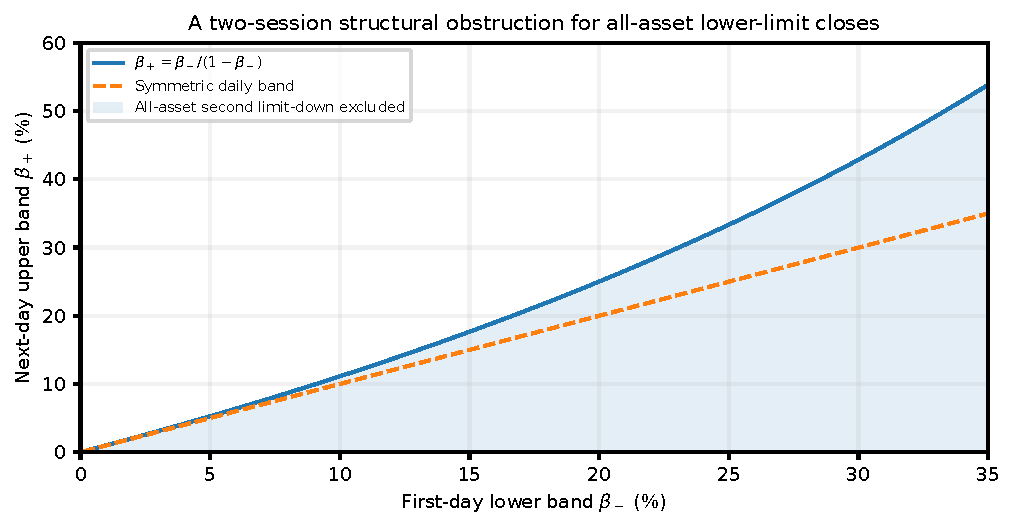
\includegraphics[width=.73\linewidth]{figures/multiday_fullbreadth_obstruction.pdf}
 \caption{\textbf{Parameter region in which the second all-asset lower-limit close is ruled out.} The region beneath the curve satisfies $(1+\beta_+)(1-\beta_-)\le1$. Symmetric proportional bands lie strictly inside this region. This is a conditional invariant-region result, not a model of exchange-wide order queues.}\label{fig:streak-full-obstruction}
\end{figure}
\begin{figure}[tbp]\centering
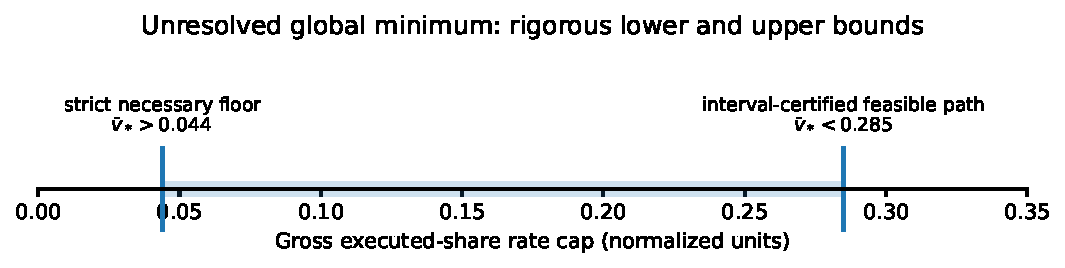
\includegraphics[width=.80\linewidth]{figures/v7_minimum_rate_bracket.pdf}
\caption{\textbf{What is and is not optimized.} A strict rate floor from the existing quadratic systemic bound and a certified feasible execution path bracket the unknown global minimum $\bar v_*$. The interval is a logical admissibility bracket, not a statistical confidence interval.}\label{fig:v7bracket}
\end{figure}
\begin{figure}[tbp]\centering
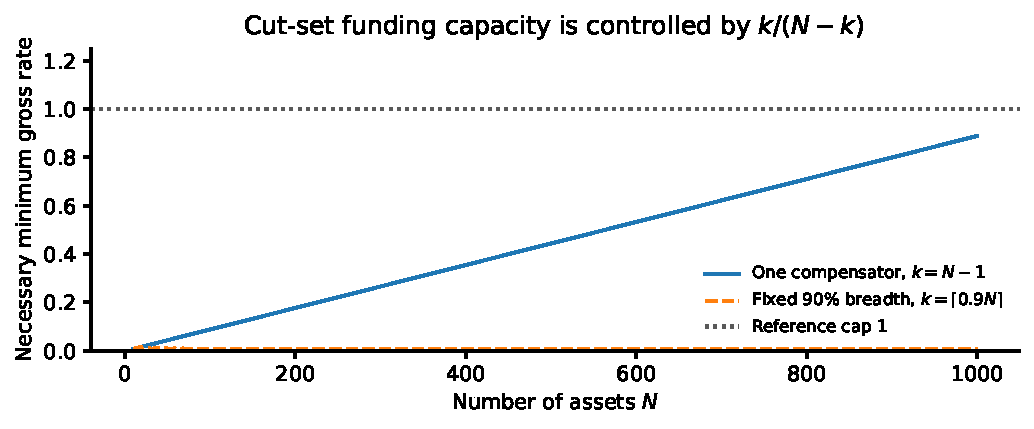
\includegraphics[width=.80\linewidth]{figures/v7_cut_capacity_N.pdf}
\caption{\textbf{A funding-capacity constraint that grows with the falling majority.} The necessary second-day rate in the main manuscript increases as $k/(N-k)$ when a single asset absorbs the net matched dollars of an expanding majority. This does not prove that a feasible market exists at every plotted $N$.}\label{fig:v7cutN}
\end{figure}
\begin{figure}[tbp]\centering
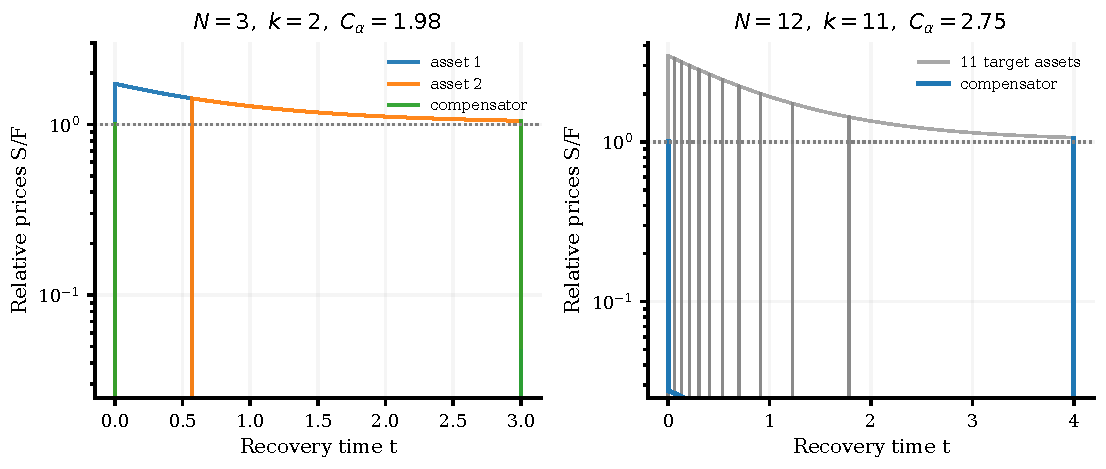
\includegraphics[width=.98\linewidth]{figures/closed_flow_price_paths.pdf}
\caption{\textbf{Constructed price paths with terminally closed dollar flows.} For $N=3$ and $N=12$, one compensating asset ends above its initial value, while the other $N-1$ prices fall by the common target log loss $L=3$. Logarithmic vertical scales keep near-zero prices visible. Kinks and jumps are permitted control pulses, not simulated exchange events.}\label{fig:paths}
\end{figure}
\begin{figure}[tbp]\centering
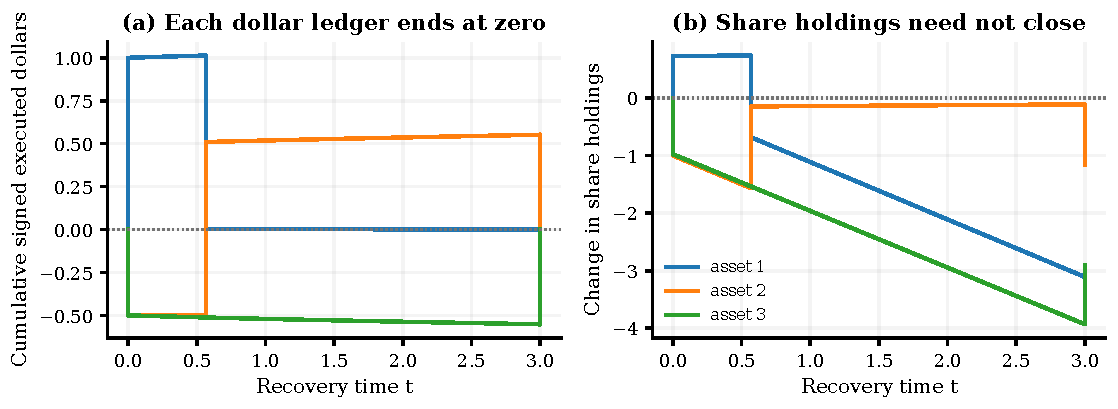
\includegraphics[width=.97\linewidth]{figures/dollar_vs_share_closure.pdf}
\caption{\textbf{Net executed dollars are not net shares.} A separate $N=3$, $k=2$, $T=3$, $L=5$ witness has $X_i(T)=0$ for every asset (left), but its net share positions generally differ from zero (right). Initial share inventories must cover gross sales; transaction closure alone does not supply them.}\label{fig:closure}
\end{figure}
\begin{figure}[tbp]\centering
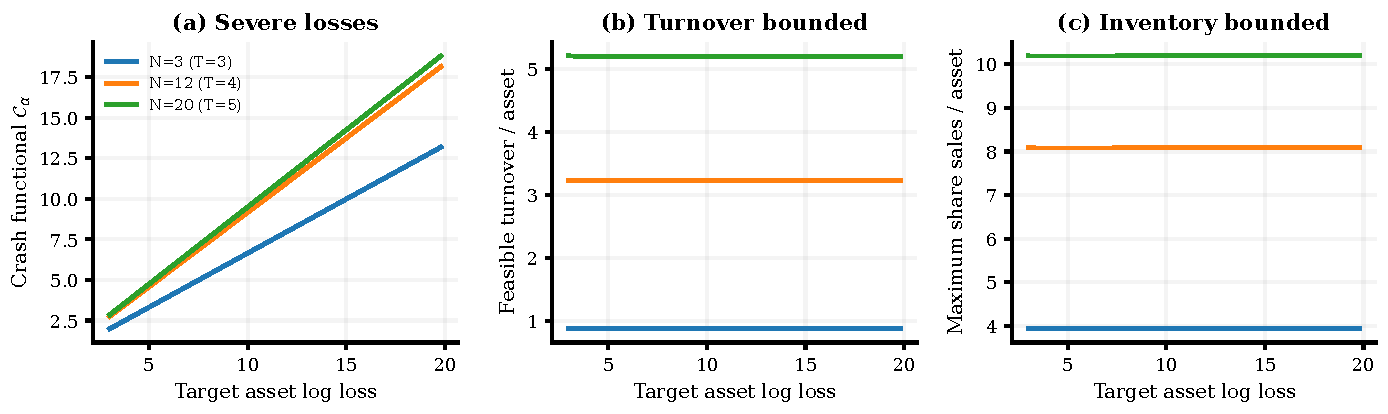
\includegraphics[width=.99\linewidth]{figures/finite_resources_severe_crashes.pdf}
\caption{\textbf{Increasing crisis severity with bounded \emph{feasible} resources.} Selected $N=3,12,20$ construction families use $k=N-1$ and horizons $T=3,4,5$, respectively. As the terminal target-price log loss increases, achieved $\mathcal C_\alpha$ rises (left), whereas the particular paths' turnover per asset (center) and largest cumulative share sale (right) remain bounded. The different horizons and prices are model choices, not a cross-market calibration or an optimum.}\label{fig:finite}
\end{figure}
\begin{figure}[tbp]\centering
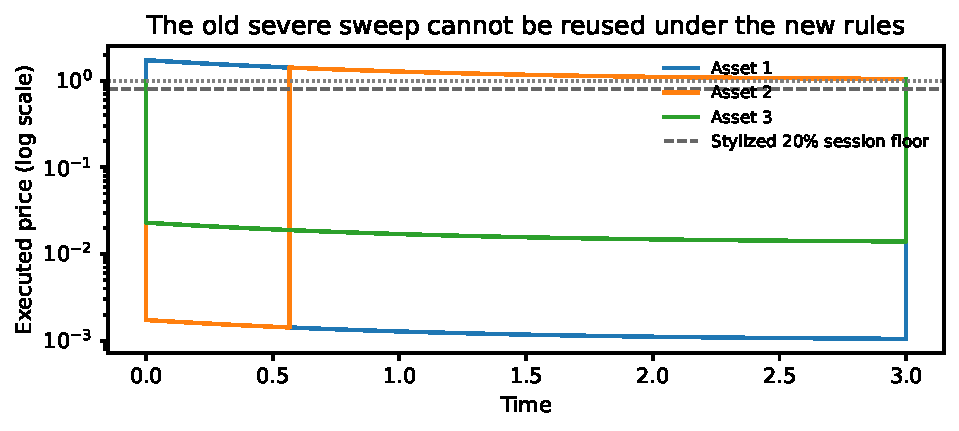
\includegraphics[width=.75\linewidth]{figures/old_pulse_path_fails_limits.pdf}
\caption{\textbf{Diagnostic rejection of an old severe path under new execution restrictions.} The $N=3$, $p=0$ severe-dollar-closed witness from the unrestricted model crosses a stylized one-session 20\% lower band and includes nonzero instantaneous pulses. Its exact closed dollar ledger therefore \emph{does not} certify reachability under either a finite gross rate or the price-limit protocol.}\label{fig:oldrejected}
\end{figure}
\end{document}
